% ==============================================================================
\section{Background}
% ------------------------------------------------------------------------------
\begin{frame}{Modelling Research Question}
  \begin{itemize}
    \item \bfcolor{Research Question:}
      impact of \textbf{hotspot} vs \textbf{non-hotspot}\\
      \covid vaccine prioritization in Ontario
      \bigskip
    \item \bfcolor{Transmission Model:}
    \begin{itemize}
      \item 513 FSA (first 3 postal code) $\rightarrow$ \textbf{10 deciles} by cases
      \item \textbf{12 age} groups: [0--11, 12--15, 16--39, 40--44, 45--49, \dots, 80+]
      \item \textbf{2 contact types}: home, travel%
        \footnote{travel = work + school + transport + leisure + other}
      \item \covid stuff \dots
    \end{itemize}
  \end{itemize}
\end{frame}
% ------------------------------------------------------------------------------
\begin{frame}{513 FSA by Cumulative \Covid Cases Deciles}
  \centering\scalebox{.9}{\begin{tikzpicture}
  \node at (-5.5,+1.5) {\includegraphics[width=5cm]{Brown2021a}};
  \node at ( 0.0, 0.0) {\includegraphics[width=8cm]{Brown2021b}};
  \node at (+4.0,-1.0) {\includegraphics[width=6cm]{Brown2021c}};
  \node at (-6.7,-1.2) {\includegraphics[width=2cm]{Brown2021x}};
\end{tikzpicture}}
  \footnote{Brown 2021}
\end{frame}
% ------------------------------------------------------------------------------
\begin{frame}{\Covid Cases by Decile (t)}
  \centering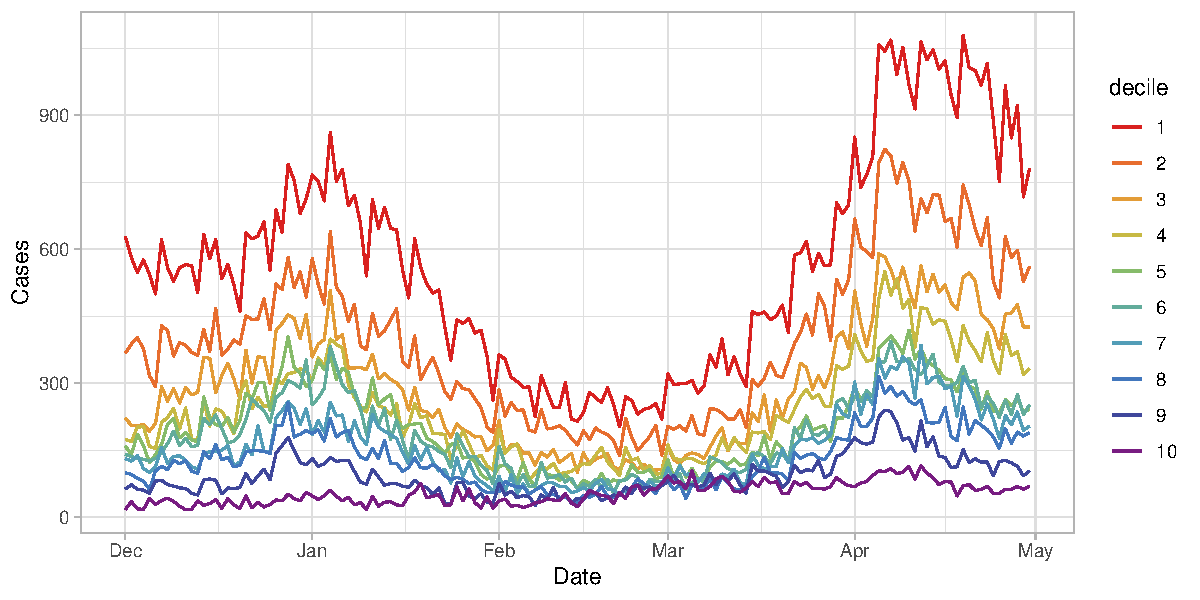
\includegraphics[height=0.85\textheight]{Yg}
\end{frame}
% ------------------------------------------------------------------------------
\begin{frame}{Objective}
  Develop a \textbf{mixing matrix}
  (number of contacts formed, and with whom)
  stratified by:
  \par\bigskip
  \begin{minipage}{.33\linewidth}
    \begin{itemize}
      \item self decile, $g$
      \item self age, $a$
    \end{itemize}
  \end{minipage}%
  \begin{minipage}{.33\linewidth}
    \begin{itemize}
      \item other decile, $g'$
      \item other age, $a'$
    \end{itemize}
  \end{minipage}%
  \begin{minipage}{.33\linewidth}
    \begin{itemize}
      \item contact type, $y$
      \item calendar month, $t$
    \end{itemize}
  \end{minipage}
  \par\bigskip
  Dimensions: $10 \times 12 \times 10 \times 12 \times 2 \times t$
  \par\bigskip
  Two versions:
  \begin{itemize}
    \item $X$: total number of contacts in the model
    \item $\chi$: contacts formed per person,\quad
    $\chi = X / P$
  \end{itemize}
\end{frame}
% ------------------------------------------------------------------------------
\begin{frame}{Methods Overview}
  \begin{enumerate}
    \item Contact Rates \& Age Mixing
    \item Mobility Patterns
    \item Complete Mixing
  \end{enumerate}
\end{frame}
% ==============================================================================
\section{Contact Rates \& Age Mixing}
% ------------------------------------------------------------------------------
\begin{frame}{\Polymod Contact Matrices, for Canada (Prem 2017)}
  \centering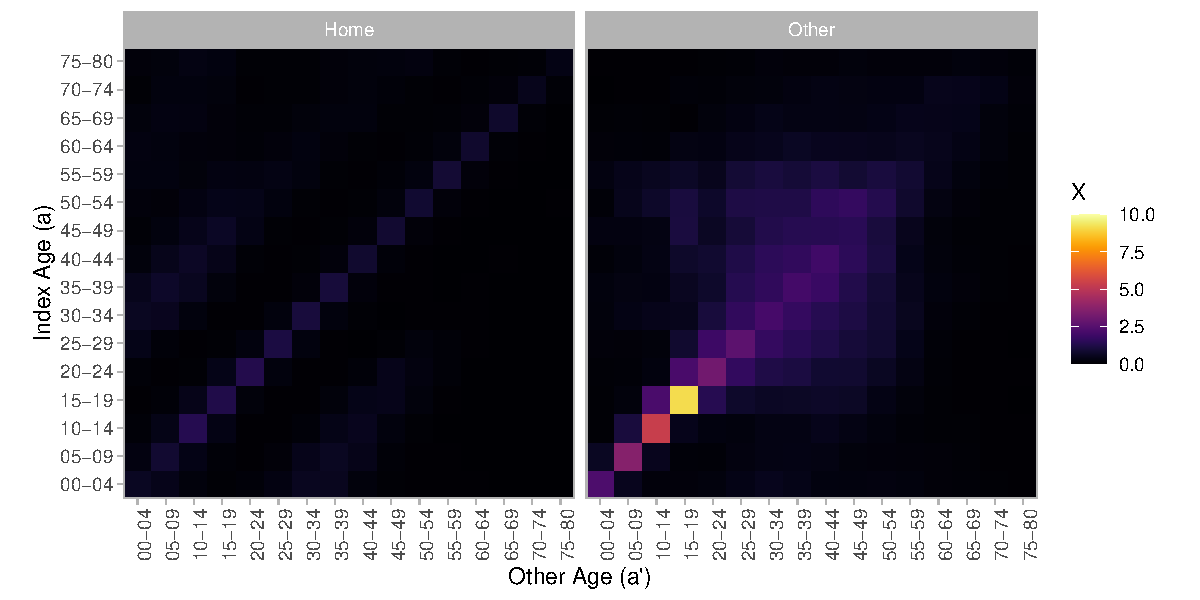
\includegraphics[height=0.85\textheight]{canada}
\end{frame}
%% ------------------------------------------------------------------------------
%\begin{frame}{\Polymod Contact Matrices, for Canada (Prem 2017): Original}
%  \centering\includegraphics[width=\linewidth]{canada-full}
%\end{frame}
% ------------------------------------------------------------------------------
\begin{frame}{Age Mixing: Three Challenges}
  \begin{enumerate}
    \item \Polymod study did not include Canada $\rightarrow$ Prem 2017
    \item Each decile: unique age distribution
    \item Age stratification not aligned
  \end{enumerate}
\end{frame}
% ------------------------------------------------------------------------------
\begin{frame}{Age Mixing 1: Canada-Specific}
  Prem et al. (2017): project \polymod contact matrices onto 152 countries, using:
  \begin{itemize}
    \item age pyramid $\rightarrow$ all types
    \item labour force participation $\rightarrow$ work
    \item school participation \& teacher-student ratio $\rightarrow$ school
    \item household age structure \& socio-demographic factors $\rightarrow$ home
  \end{itemize}
\end{frame}
% ------------------------------------------------------------------------------
\begin{frame}{Age Mixing 2: Decile Age Distributions}
  \centering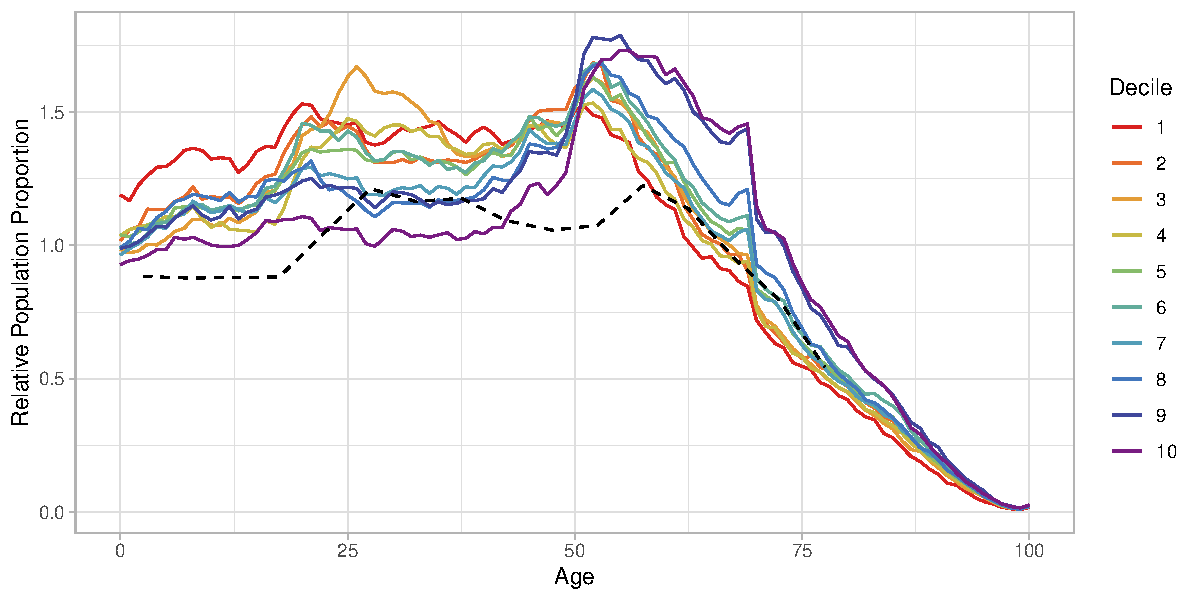
\includegraphics[height=0.85\textheight]{Pga}
\end{frame}
% ------------------------------------------------------------------------------
\begin{frame}{Age Mixing 2: \Polymod
  \only<1>{$\epsilon$ Approximation}%
  \only<2>{Original}%
  \only<3>{$\epsilon$ Approx $-$ Original}}
  \centering
  \only<1>{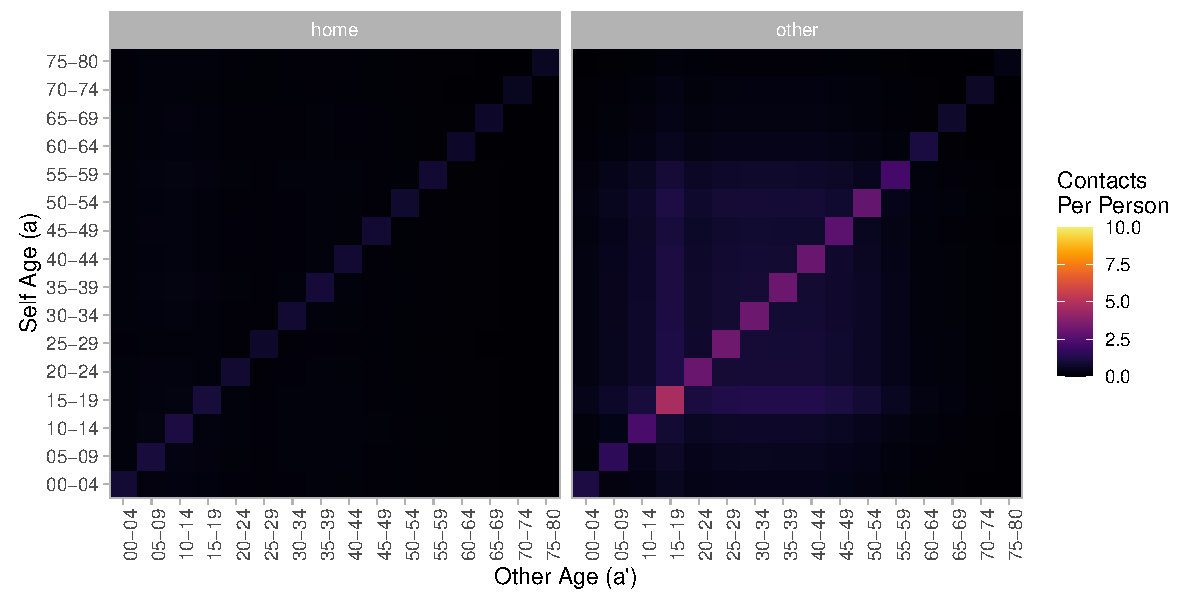
\includegraphics[height=0.85\textheight]{canada-eps}}%
  \only<2>{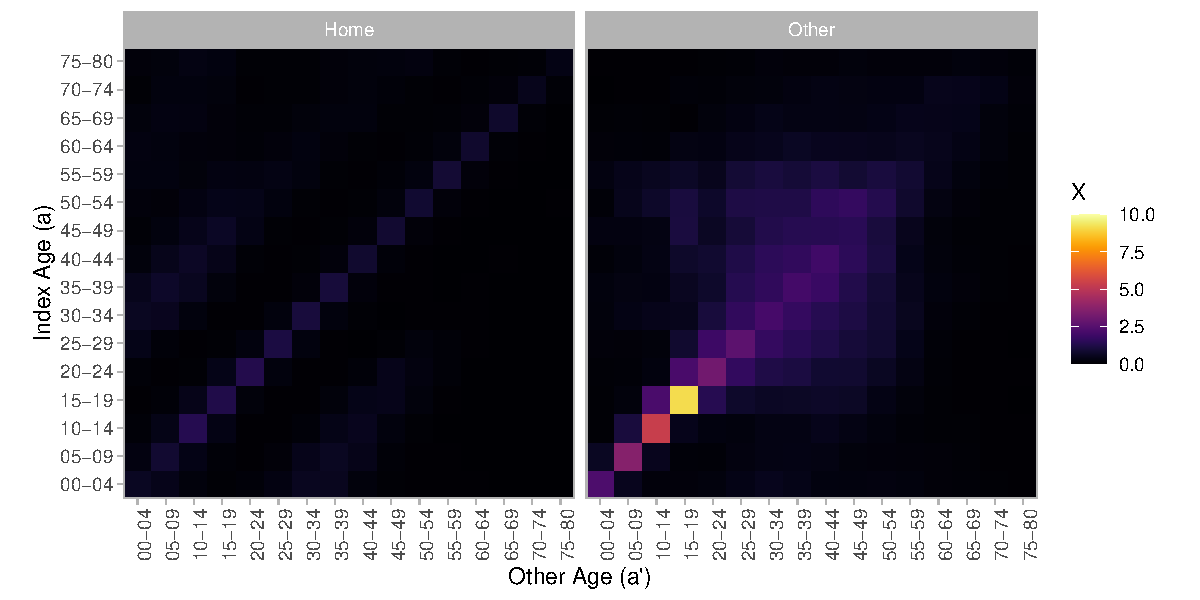
\includegraphics[height=0.85\textheight]{canada}}%
  \only<3>{\includegraphics[height=0.85\textheight]{canada-diff}}
\end{frame}
% ------------------------------------------------------------------------------
\begin{frame}{Age Mixing 3: Re-stratified Age by Interpolation}
  \centering\includegraphics[height=0.85\textheight]{C-interp}
\end{frame}
% ------------------------------------------------------------------------------
\begin{frame}{Contact Rates: Forced Scaling by Decile}
  \centering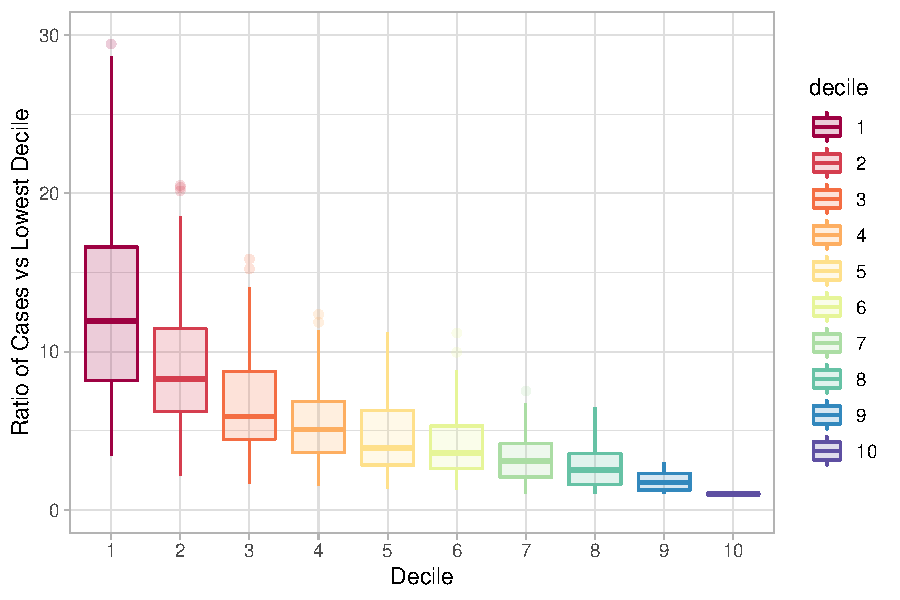
\includegraphics[height=0.85\textheight]{RYg}
\end{frame}
% ==============================================================================
\section{Mobility Patterns}
% ------------------------------------------------------------------------------
\begin{frame}{Mobility Data}
  \begin{itemize}
    \item \ttilde 2\,\% devices in each FSA
    \item For each device:
    \begin{itemize}
      \item Define \textbf{Home} FSA
      \item Count \textbf{Visits} to other FSA per day (2h+)
    \end{itemize}
    \item Average \# devices per FSA per day:
    \begin{itemize}
      \item at Home, $H_{g}$
      \item Visited other FSA, $V_{gg'}$
    \end{itemize}
    \item Repeat by calendar month, $t$
  \end{itemize}
\end{frame}
% ------------------------------------------------------------------------------
\begin{frame}{Mobility Data: Unbiased Sample?}
  \only<1,3>{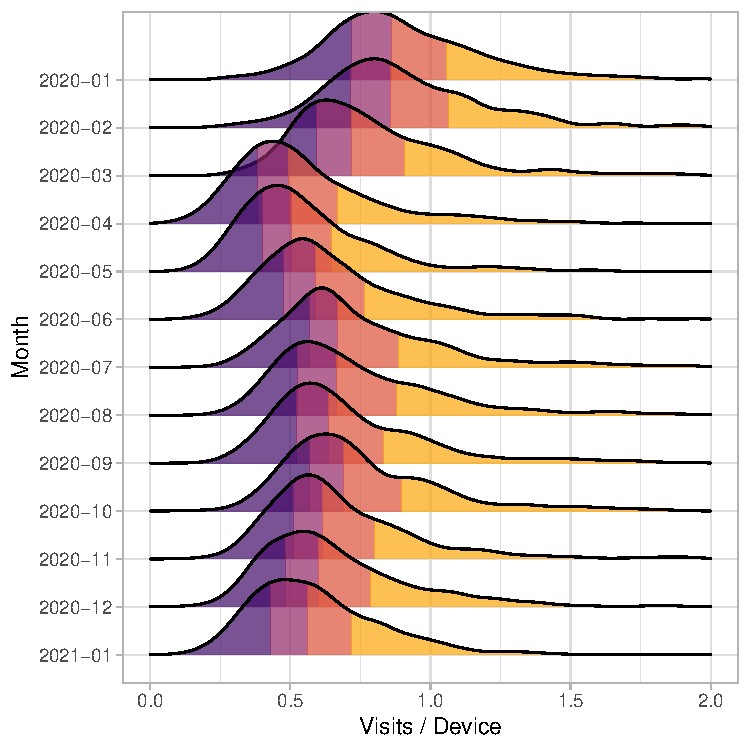
\includegraphics[height=0.85\textheight]{devices-n-month-ratio}}%
  \only<2>{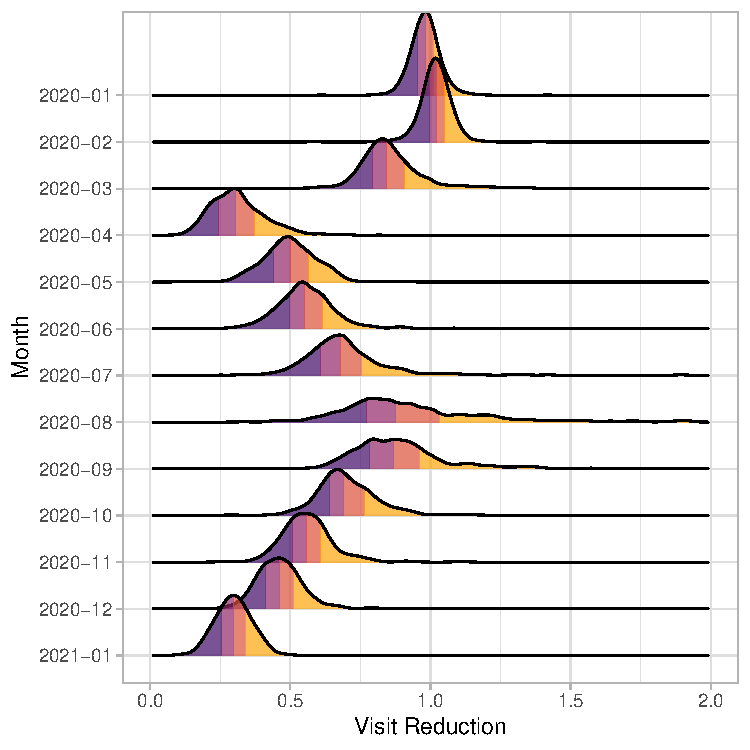
\includegraphics[height=0.85\textheight]{devices-r-month-visit}}%
  \only<2>{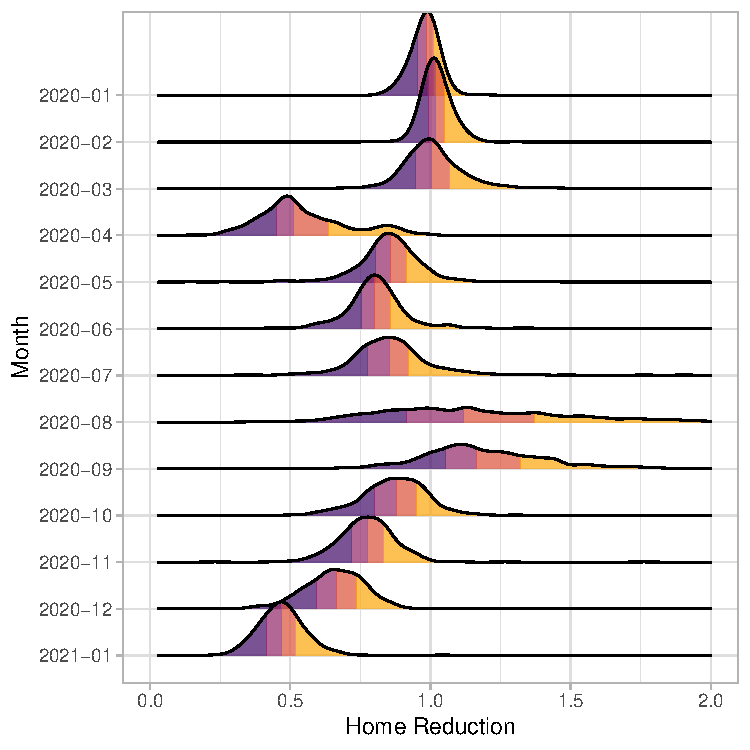
\includegraphics[height=0.85\textheight]{devices-r-month-home}}%
  \only<3>{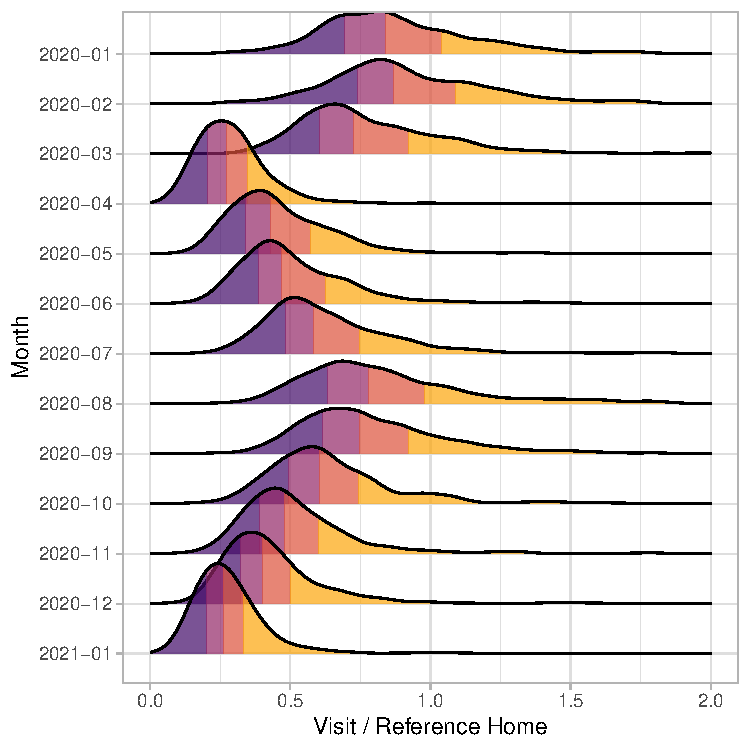
\includegraphics[height=0.85\textheight]{devices-r-month-rx}}
\end{frame}
% ------------------------------------------------------------------------------
\begin{frame}{Mobility Data: Assumptions}
  \textbf{Problem 1:} Visits ($V_{gg'}$) per device ($H_{g}$) does not reflect mobility reduction
  \par\medskip
  \textbf{Solution 1:} Use denominator ($H_{g'}$) from REF period ($t_0$: Jan--Feb 2020)
  \par\bigskip\bigskip
  \textbf{Problem 2:} Unobserved devices (98\%) less mobile
  \par\medskip
  \textbf{Solution 2:} Assume $\phi = 0.9$ as mobile
  \par\bigskip\bigskip
  \textbf{Define:} $B_{gg't} = V_{gg't} / H_{gt_0} \left[1 + \phi \left(P_{g} - H_{gt_0} \right)\right]$
\end{frame}
% ------------------------------------------------------------------------------
\begin{frame}{Mobility Matrix, $B_{gg'}$ (REF)}
  \centering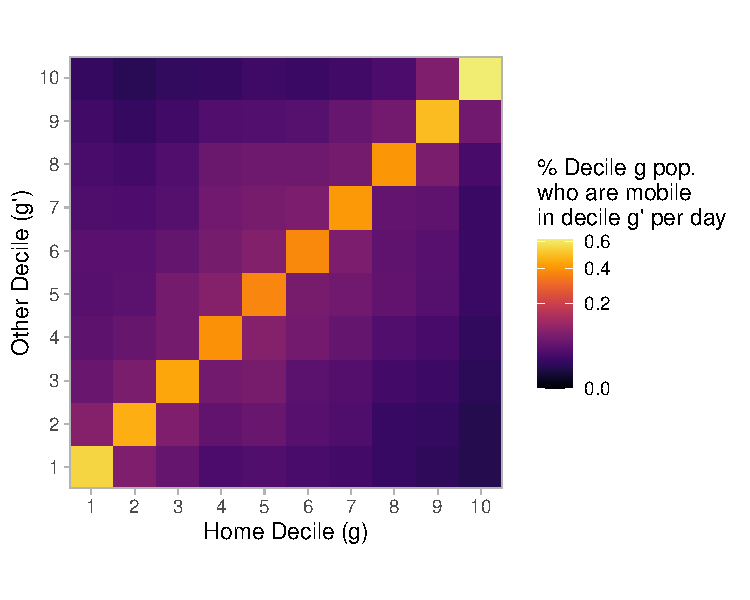
\includegraphics[height=0.85\textheight]{Bgg}
\end{frame}
% ------------------------------------------------------------------------------
\begin{frame}{Mobility Matrix, $B_{gg'}(t)$}
  \centering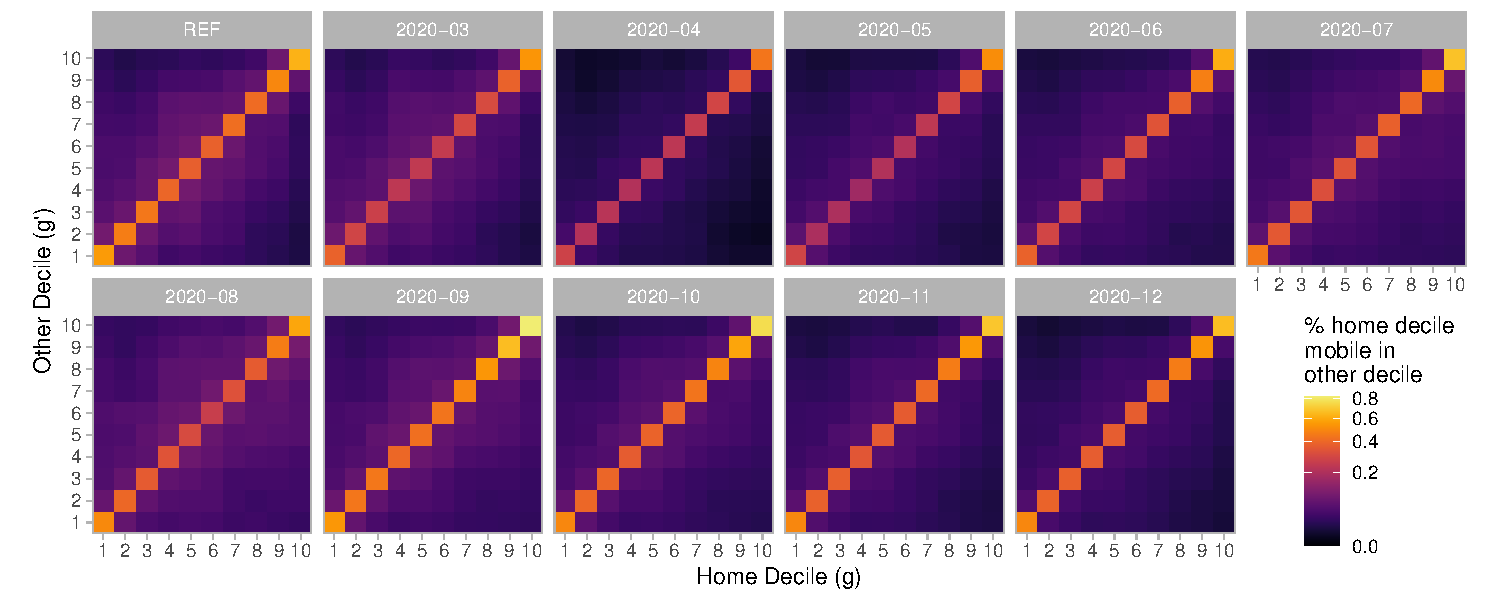
\includegraphics[width=\linewidth]{Bggt}
\end{frame}
% ==============================================================================
\section{Complete Mixing}
% ------------------------------------------------------------------------------
\begin{frame}{Mixing Pools Model:
  \only<2>{home contacts}%
  \only<3>{others visiting my decile}%
  \only<4>{others visiting same decile as me}%
  \only<5>{others visiting same decile as me}%
  }
  \centering
  \only<1>{\def\bxx{fx}\def\bxh{fx}\def\bxa{fx}\def\bxb{fx}\def\bxc{fx}}
  \only<2>{\def\bxx{}{}\def\bxh{fx}\def\bxa{}{}\def\bxb{}{}\def\bxc{}{}}
  \only<3>{\def\bxx{}{}\def\bxh{}{}\def\bxa{fx}\def\bxb{}{}\def\bxc{}{}}
  \only<4>{\def\bxx{}{}\def\bxh{}{}\def\bxa{}{}\def\bxb{fx}\def\bxc{}{}}
  \only<5>{\def\bxx{}{}\def\bxh{}{}\def\bxa{}{}\def\bxb{}{}\def\bxc{fx}}
  \scalebox{0.8}{\footnotesize\definecolor{GX}{HTML}{999999}
\begin{tikzpicture}[x=6ex,y=6ex]
 \useasboundingbox (-6,-5) rectangle (+6,+4);
  \node[align=center] at (-5.5,+3) {home\\pools};
  \node[align=center] at (-5.5, 0) {FSA\\populations};
  \node[align=center] at (-5.5,-4) {travel\\pools};
  \node[align=center] at (+5.5, 0) {\dots};
  \node[ pop={12ex}{G1},bx] (A)  at (-3, 0) {1};
  \node[ pop={12ex}{G2}]    (B)  at ( 0, 0) {2};
  \node[ pop={12ex}{G3},bx] (C)  at (+3, 0) {3};
  \node[pool={12ex}{G1},bx] (Ah) at (-3,+3) {1\\home};
  \node[pool={12ex}{G2}]    (Bh) at ( 0,+3) {2\\home};
  \node[pool={12ex}{G3},bx] (Ch) at (+3,+3) {3\\home};
  \node[pool={12ex}{GX}]    (At) at (-3,-4) {1\\travel};
  \node[pool={12ex}{GX}]    (Bt) at ( 0,-4) {2\\travel};
  \node[pool={12ex}{GX}]    (Ct) at (+3,-4) {3\\travel};
  \draw[arrow,G1,->,bx] (A) edge (Ah);
  \draw[arrow,G2,->]    (B) edge node[left]{(c)} (Bh);
  \draw[arrow,G3,->,bx] (C) edge (Ch);
  \draw[arrow,G1,->,bx] (A) edge (At);
  \draw[arrow,G2,->]    (B) edge[bend left =10] node[above left ]{(a)} (At);
  \draw[arrow,G3,->,bx] (C) edge[bend left =10] (At);
  \draw[arrow,G1,->,bx] (A) edge[bend right=10] (Bt);
  \draw[arrow,G2,->]    (B) edge node[left]{(b)} (Bt);
  \draw[arrow,G3,->,bx] (C) edge[bend left =10] (Bt);
  \draw[arrow,G1,->,bx] (A) edge[bend right=10] (Ct);
  \draw[arrow,G2,->]    (B) edge[bend right=10] node[above right]{(a)} (Ct);
  \draw[arrow,G3,->,bx] (C) edge (Ct);
\end{tikzpicture}
}
\end{frame}
% ------------------------------------------------------------------------------
\begin{frame}{Mixing Pools: Math}
  Total type $y$ contacts made available by age group $a$ in decile $g$:\quad
  $Q_{gay} = P_{ga} \times C_{gay}$
  \par\bigskip
  \paragraph{Home Contacts:}
  \begin{itemize}
    \item 100\% $Q_{gay}$ with same decile
    \item $X_{gg'}$ mixing by decile $g$: identity matrix
    \item $X_{aa'}$ mixing by age $a$: from $\epsilon$-\polymod ``home''
  \end{itemize}
\end{frame}
% ------------------------------------------------------------------------------
\begin{frame}{Mixing Pools: Math}
  \paragraph{Other Contacts:}
  \begin{itemize}
    \item $B_{gg'}$\,\% of $Q_{gay}$ formed in (not with) $g'$
    \item Within $g^*$ travel pool:
    \begin{itemize}
      \item Total contacts available (denominator): $T_{g^*} = \sum_{g} B_{gg^*} Q_{gay}$
      \item $X_{gg'}^{g^*}$ mixing by decile $g$: proportionate
      \item $X_{aa'}^{g^*}$ mixing by age $a$: from $\epsilon$-\polymod ``travel''
    \end{itemize}
    \item Total mixing across all travel pools: $\sum_{g^*} X_{gag'a'y}^{g^*}$
    \item Assume remaining contacts ($1-\sum_{g'} B_{gg'}$) formed with local travel pool
  \end{itemize}
\end{frame}
% ------------------------------------------------------------------------------
\begin{frame}{Decile Mixing: No Contact Scaling}
  \centering\includegraphics[height=0.85\textheight]{Ciggy-1}
\end{frame}
% ------------------------------------------------------------------------------
\begin{frame}{Decile Mixing: With Contact Scaling}
  \centering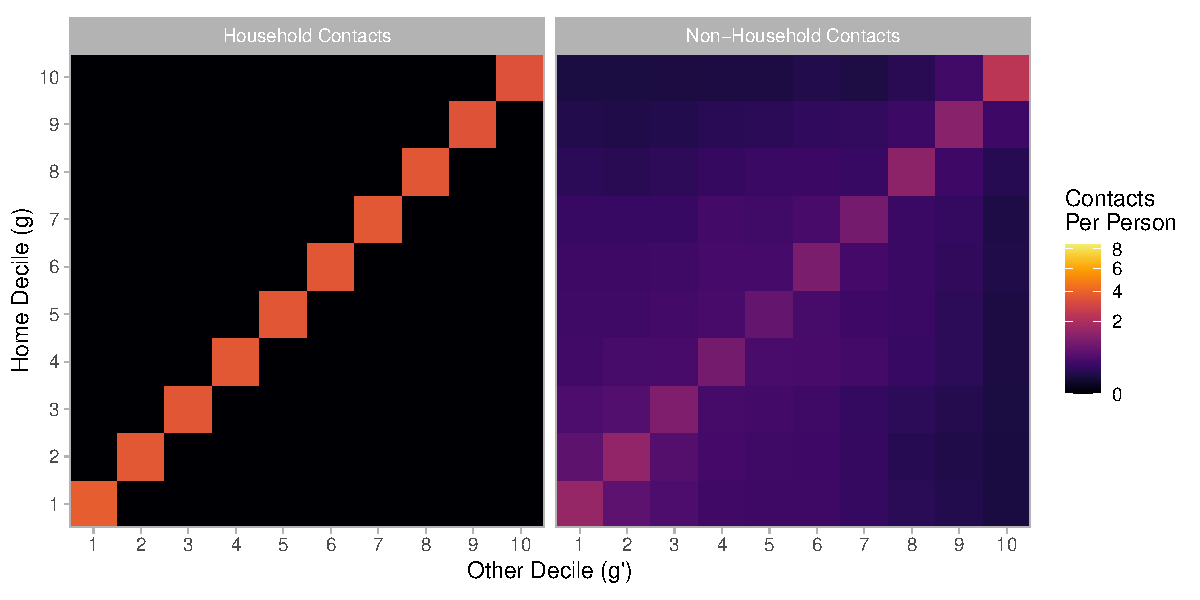
\includegraphics[height=0.85\textheight]{Ciggy}
\end{frame}
% ------------------------------------------------------------------------------
\begin{frame}{Age Mixing}
  \centering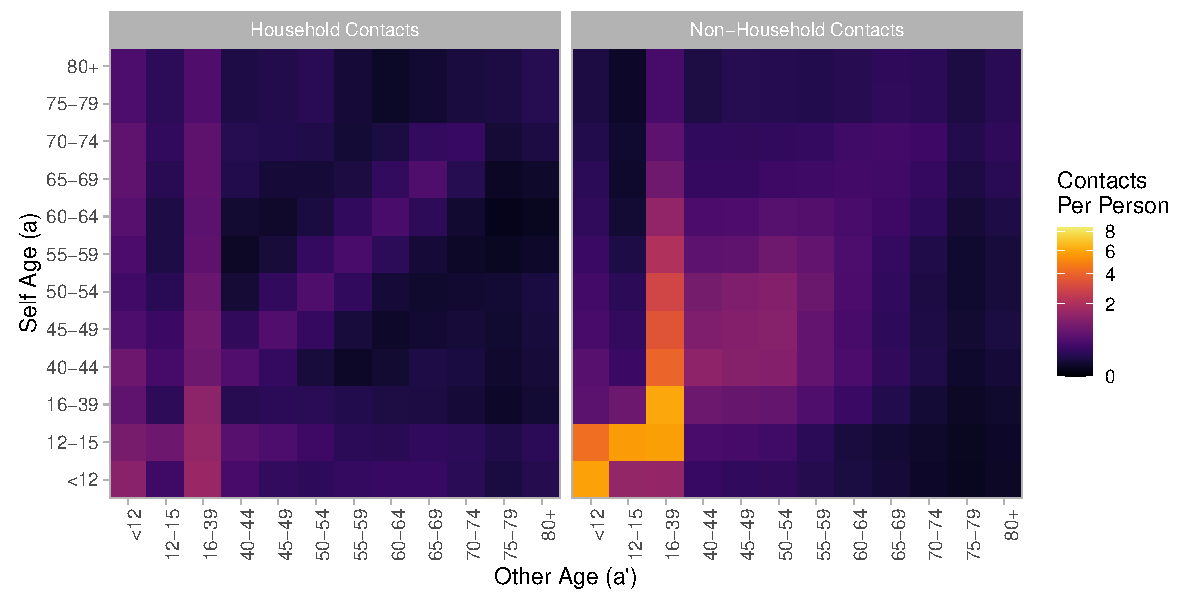
\includegraphics[height=0.85\textheight]{Ciaay}
\end{frame}